\begin{figure}[!htb]
\centering
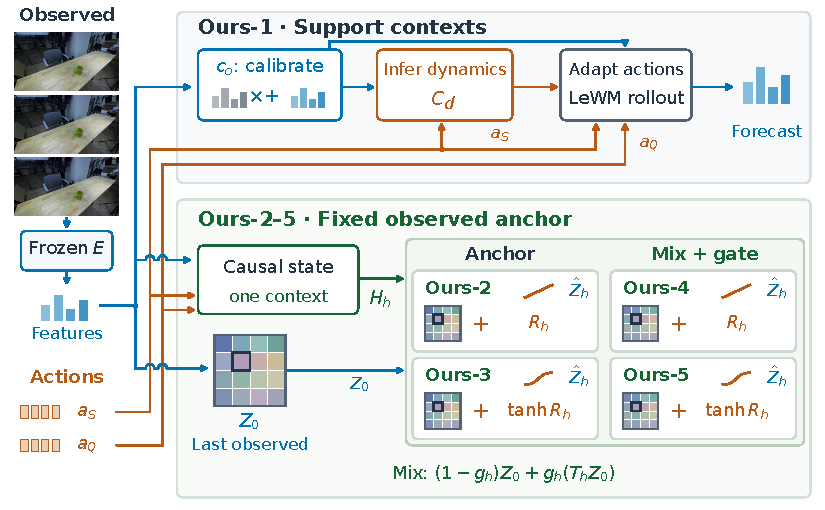
\includegraphics[width=\linewidth]{generated/editorial/method_family.pdf}
\caption[Method family overview.]{\textbf{Two ways to use observed evidence.} Ours-1 calibrates history with $c_o$, then infers $c_d$ from corrected transitions and past actions to condition LeWM. Ours-2--5 build a spatial state with past-only transition context and retain the last observed grid $Z_0$. Columns toggle gated row-stochastic feature mixing; rows toggle innovation bounding. Each cell specifies the future-feature forecast $\hat Z_h$. Recorded DROID images are unchanged (CC BY 4.0); latent colors are schematic. Shared interfaces do not imply shared weights, representations, or evaluation protocols. Detailed architectures and simulator-only planning appear in Appendices~\ref{app:spatial-development} and~\ref{app:original-context-study}.}
\label{fig:method-family}
\end{figure}
